\chapter{Statistiche Finali}\label{chap:final-stats}
In questo capitolo verranno analizzate alcune statistiche estratte dal Product Backlog.

\medbreak
Nella Figura \ref{fig:commits} sottostante si può osservare l'andamento durante tutto il periodo di sviluppo del progetto. Solamente considerando i commit, il processo è iniziato gradualmente, per poi entrare nel vivo dell'implementazione, e infine lasciare più spazio alle correzioni finali. Questo si allinea con le considerazioni fatte nella retrospettiva dello sprint 10 in cui, grazie alla buona gestione di progetto, c'è stato tempo per le correzioni finali.

\begin{figure}[H]
    \centering
    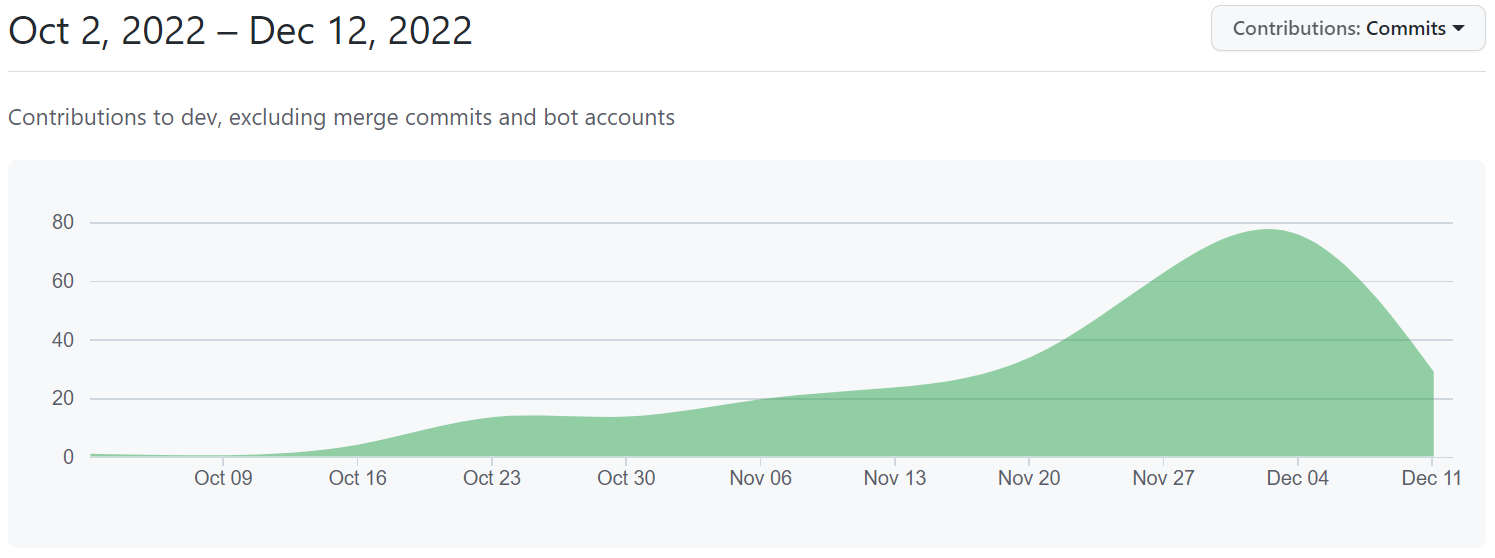
\includegraphics[width=\textwidth]{process/Img/charts/project-commits.png}
    \caption{Commit totali nel repository}
    \label{fig:commits}
\end{figure}

Nel grafico sottostante (Figura \ref{fig:stats-items}) si possono osservare gli item dei vari backlog in ogni sprint. Come si può notare, il carico di lavoro combacia con quanto detto in precedenza. C'è da osservare inoltre che, essendo gli item raffinati, è normale che ce ne siano di più verso la fase finale.
\begin{figure}[H]
    \centering
    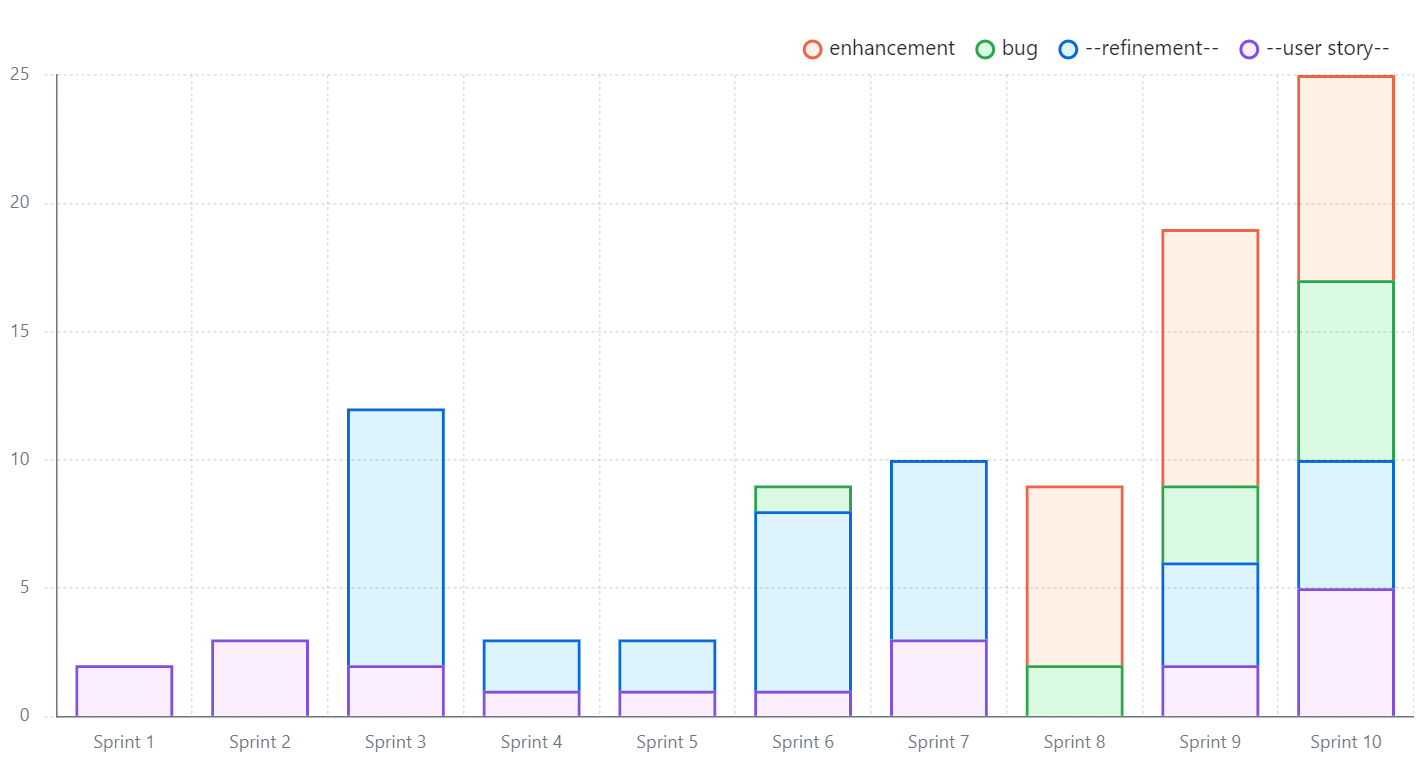
\includegraphics[width=\textwidth]{process/Img/charts/items-for-sprint.png}
    \caption{Items portati a termine in ogni sprint}
   \label{fig:stats-items}
\end{figure}

Dall'ultimo grafico (Figura \ref{fig:stats-dimension}) si può evincere come il raffinamento delle user stories sia stato fatto correttamente. Infatti queste si trovano nella parte sinistra del grafico, in cui gli item hanno più story points. Invece, i raffinamenti e gli enhancements vanno a incrementare di numero scendendo di complessità.
\begin{figure}[H]
    \centering
    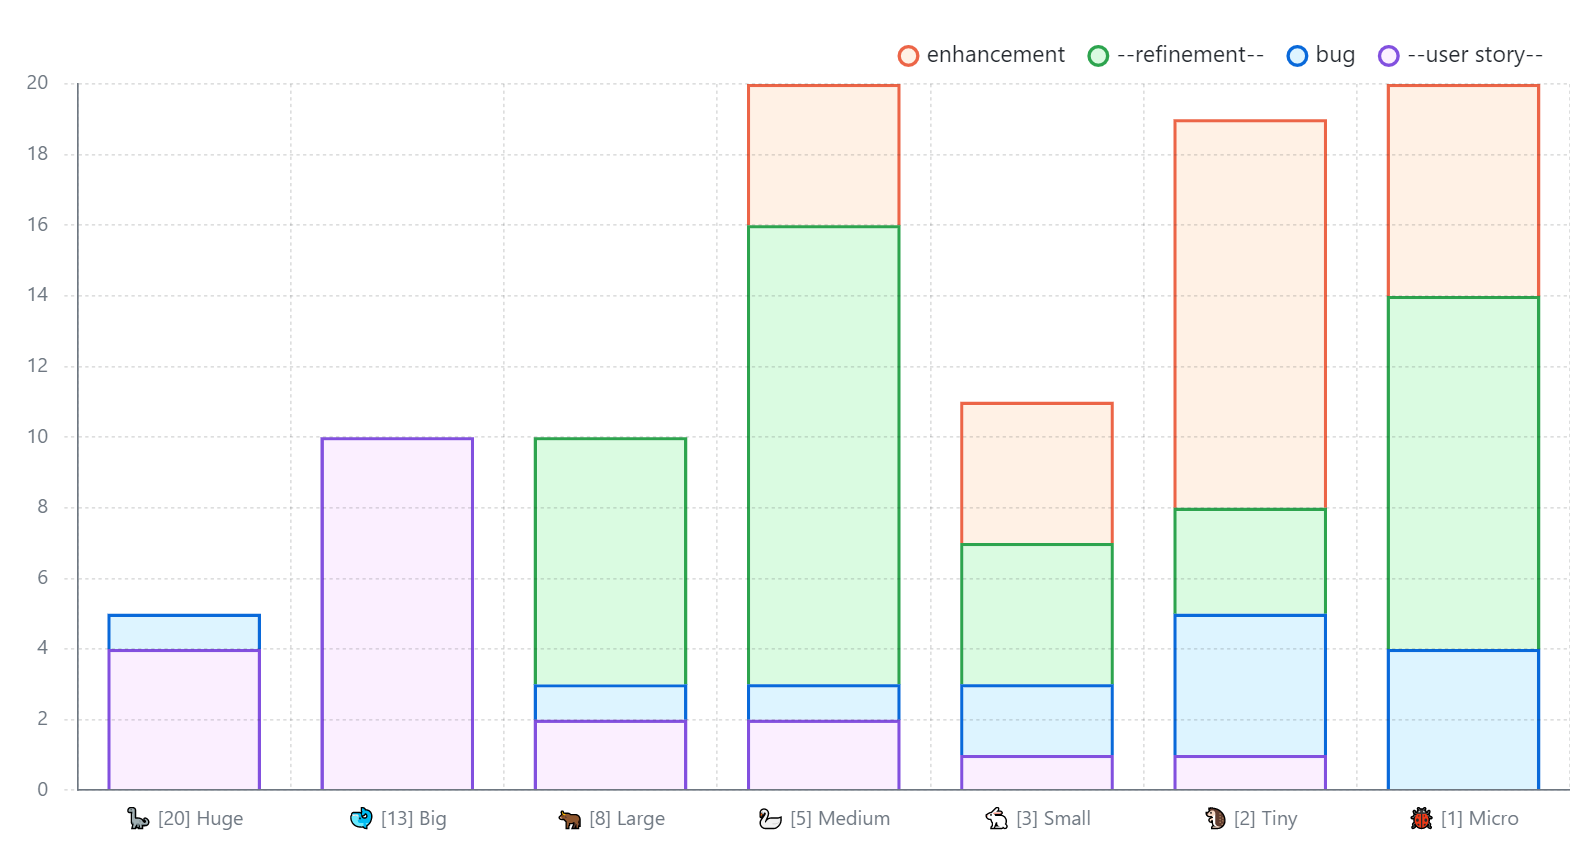
\includegraphics[width=\textwidth]{process/Img/charts/items-for-size.png}
    \caption{Dimensione dei vari item}
    \label{fig:stats-dimension}
\end{figure}